\chapter{Design and Implementation}

\section{Modelling}

\subsection{The Protocol}
% TODO: (e.g., cite this paper: http://ilyasergey.net/papers/paxos-register-extended.pdf)
For mechanising the proof of Paxos in Disel, we followed the approach highlighted
in the Disel section of Chapter 2 by first writing and testing the code for
the protocol before writing the proofs. Applying this approach meant
we needed to come up with the state transition system and the inductive invariant
for the protocol which we will encode in Disel. Before coming up with these things
though, we decided to simplify the actual simple paxos protocol that we will prove.

The goal of this simplification was to reduce the amount of things that we will need
prove in Disel by actually focusing on the 'core' parts of the protocol which
lead to consensus being achieved. The 'convenience' parts of the protocol, like
the sub phase of informing the learner, aren't necessary for consensus being
achieved in the global state and can also be proved separately after we have
finished proving the 'core' parts of the protocol.

In order to adapt the protocol and focus on the 'core' parts, the first thing
we did was to do away with the 'Learning the Chosen Value' phase of simple paxos.
This is the phase where once an acceptor has accepted a proposal, it then informs
a leaner by sending it an accepted request. We decided against proving this
because we can use the inductive invariant to check the global state of the system.
The inductive invariant allows to check when a majority of acceptors have
accepted a proposal and what proposal each of them has accepted. Thus, we can know
from the inductive invariant when consensus has been achieved by checking the values
of each of the accepted proposals.

Doing away with the learning phase also meant that we did not have to implement
a learner in our protocol as the role of the learner (detecting that consensus
has been achieved) is performed by the inductive invariant.
The learner is useful in actual paxos implementations as
it can detect when consensus is achieved and can the inform the client, its
presence does not change how consensus is achieved. Removing the learner simplified
our state transition diagram for the protocol as we did not have to account
for the states of the learner and also the $Phase 2b$ transition of the
accepted request.

Additionally, we decided to remove some optimisation from the protocol.
Optimisations are aspects of the protocol that improve its running time or
resource consumption but improving upon the 'mundane' way of doing the same
thing. Removing optimisations allowed us to simplify our proofs in Disel.

Firstly, we decided that a proposer, if it fails while trying to achieve
consensus with a proposal number (i.e. it receives a nack), it then does not
retry with a higher proposal number. Removing this optimisation meant we did not
have to deal with the state of a proposer where it changes the proposal number it
was initialised with. Removing this optimisation only
effects the liveness of the protocol but not its safety, as if a proposer
receives a nack, it is just an indication that it will not be able to achieve
consensus with the proposal number that it is currently using. Thus, in order
for consensus to be achieved, a proposer which is initialised with a higher
proposal number will have to successfully get promises from a quorum of acceptors.

Additionally we removed the minor optimisation of choosing a majority for
sending requests from the proposer. The proposer instead of choosing a
quorum of acceptors for sending a message, chooses the entire set of acceptors.
This does not alter the protocol as the entire set of acceptors is a valid
quorum of acceptors.

This adapated and simplified protocol allows us to focus on verifying the core
logic (the part dealing with achieving consensus) of paxos. The
optimisations and 'conveniece' that we removed can be verified separately after
the core logic has been verified.


\subsection{State Transitions}
Having adapted the protocol, we then had to create a state transition system for
the nodes in our protocol in order to encode it in Disel. For creating the states,
we need to look at what the function of each node is in the protocol at a particular
moment and what type of data it holds at that time.

A node should only be able to transition from one state to another when it either
receives or sends a message. Therefore, the data held by the node in each state
should be enough for it to be able to create the message it wants to send or to
be able to correctly process the message it receives.

We tried to minimise the number of states and transitions between them, in order
to simplify the proof in Disel. This was important because each state transition
has to be shown to hold with the invariant so reducing the state transitions,
reduces the number of proofs.

We decided that a node can either be initialised as an acceptor or a proposer.
The state transitions of each node will depend upon this intial state, so below
we will separately look at the state transition systems for the proposer and the
acceptor.

The main difference between the state transition for the acceptor and the proposer
is that the acceptor sends and receives messages from a single proposer while a
proposer has to send and receive messages from all the acceptors.


\subsubsection{Proposer}
\begin{figure}
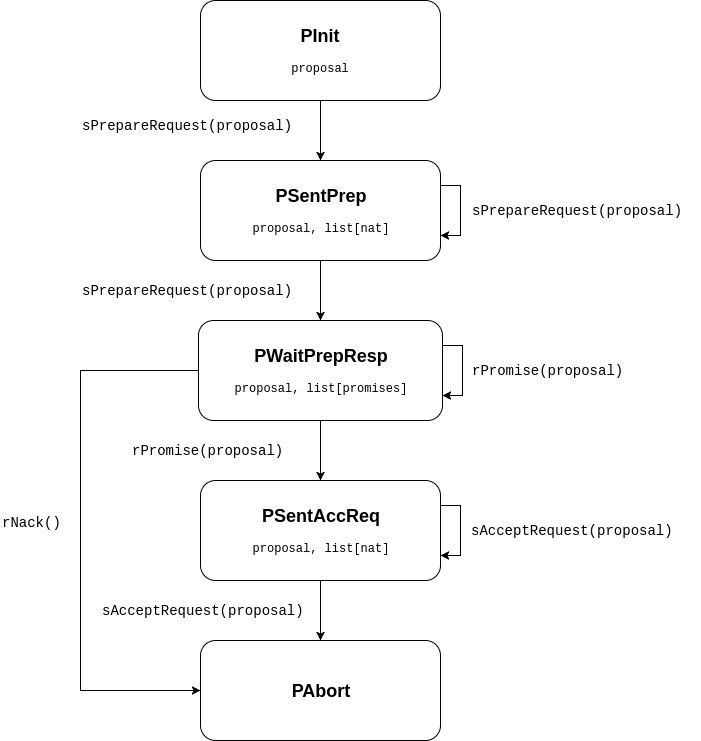
\includegraphics[width=\textwidth]{figures/proposer_state_transitions.png}
\caption{Proposer State Transition Diagram
\label{fig:myInlineFigure}}
\end{figure}

The proposer starts off in the \texttt{PInit} state where it is initialised with
a \texttt{proposal} (a custom defined data type which is tuple of two natural numbers),
$\langle p, v \rangle$.
The natural number $p$ is the proposal number and $v$ is the value that the
proposer tries to achieve consensus on. This means that the first prepare
request this proposer sends will this proposal $\langle p, v \rangle$.

The proposer then moves to the \texttt{PSentPrep} state when it starts to send prepare
requests to the acceptors. In this state, the proposer still holds the proposal
but additionally now also stores a list of natural numbers, \texttt{sent\_to}. This list stores the
natural number identifiers of the acceptors, this proposer has sent requests to.
Whenever it sends a prepare request to an acceptor, it adds the identifier of
the acceptor to this list.
The proposer remains in the \texttt{PSentPrep} state and keeps sending prepare requests
until the contents of \texttt{sent\_to} become equal to the global list \texttt{acceptors} which
holds the identifiers of all the acceptors in the system. This means the proposer
stays in this state until it has sent a prepare request to every single acceptor
in the system.

Once the proposer has sent the last prepare request, it them transitions to
the \texttt{PWaitPrepResp} state. In this state the proposer again holds a proposal and
another list \texttt{promises} which is defined as below to be a list of tuples
each containing a \texttt{nid} (a natural number identifier for a node), a boolean
and a \texttt{proposal}.

\texttt{Definition promises := seq (nid * bool * proposal).}

The proposer stays in this states and keeps receiving messages from the acceptor
until one of the following two things happen:
\begin{enumerate}
  \item It receives a nack response from the acceptor. This indicates that the
    acceptor might already have promised a proposal
    with a proposal number greater than $p$. This leads to the proposer to
    transition into the \texttt{PAbort} state. In this state the proposer basically
    gives up trying to achieve consensus using the proposal number $p$ that it was
    initialised with and completely stops sending and receiving messages. Hence,
    the proposer doesn't need to hold any data in this state.
  \item It receives a promise response from every single acceptor. When this
    happens, the proposer transitions to the \texttt{PSentAccReq} state.
\end{enumerate}

When the proposer reaches the \texttt{PSentAccReq}, it means it has received a promise
from every single acceptor and it can now start sending accept requests to each
of the acceptors in the system. In the \texttt{PSentAccReq} the proposer again stores
a list \texttt{sent\_to} to keep track of every single acceptor it has already sent the
accept request to. It also stores another \texttt{proposal} which is has the same
proposal number $p$ that the proposer was initialised with but the value $v$ is the
the value from the highest numbered proposal it received in a promise response.
In the verification section, we will look at how it determines this value by looping over
the \texttt{promises} list from the \texttt{PWaitPrepResp} state. The sending of
accept requests works similar to sending prepare requests in the
\texttt{PSentPrep} state. Finally, when the proposer finishes sending the
accept requests to all the acceptors, it transitions to the \texttt{PAbort}
state where it stops sending and receiving messages.


\subsubsection{Acceptor}
\begin{figure}
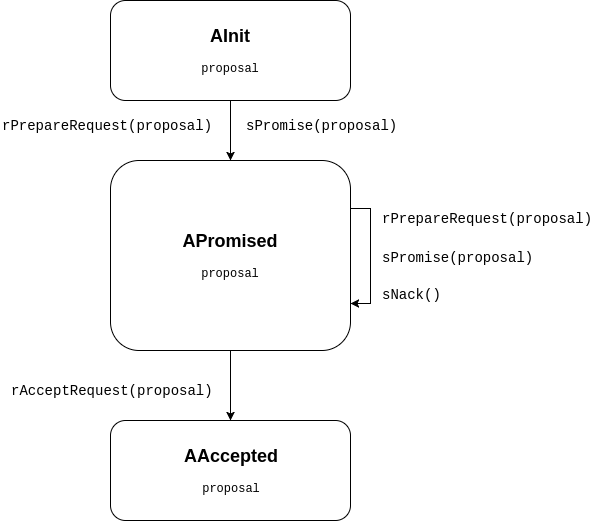
\includegraphics[width=\textwidth]{figures/acceptor_state_transitions.png}
\caption{Acceptor State Transition Diagram
\label{fig:myInlineFigure}}
\end{figure}

The Acceptor starts off in the \texttt{AInit} state. It doesn't hold any data
in this state as it is not sending any messages. It keeps listening for messages
and on receiving a prepare request message, it transitions to \texttt{APromised}
state.

In the \texttt{APromised} state, the acceptor holds a \texttt{proposal}. This is
the highest numbered proposal that it has received so far in a prepare request
message. In this state, on receiving a prepare request, if the proposal number
of the proposal in the prepare request is greater than the proposal number of
the proposal it currently holds, it updates its current state to hold the new
proposal but still remains in the \texttt{APromised} state. If the proposal
number of the proposal in the prepare request is not greater, the acceptor
sends a nack response to the proposer who sent the prepare request and does not
update its state.

In the \texttt{APromised}, on receiving an accept request, if and only if
the value of the proposal number proposal in the accept request is greater than
the proposal number of the proposal that it currently holds, it transitions to the
\texttt{AAccepted} state where it now holds the new proposal with the greater
proposal number. If the proposal number of the new proposal number is not greater,
the acceptor remains in the same state.

In the \texttt{AAccepted} state, the acceptor stops listening for and responding
to messages. This is similar to the \texttt{PAbort} state for the proposer.


\subsection{Inductive Invariant}
A critical part of proving our protocol in Disel was desiging an inductive invariant
for our adapted protocol. The inductive invariant helps ensure the correctness of
our adapted protocol enabling us to imposing requirements on the global state of the system.
For proving the correctness of paxos we found that our invariant had to capture
when consensus is achieved on a value and also that once consensus is achieved
on a particular value, further rounds of the protocol don’t change this value.

Inductive invariant means a property which when it holds for a state $s$,
it will hold for any state $s'$ reachable from $s$.

The crux of Paxos' correctness lies in the prepare phase where, before sending
the accept request, the Proposer must first set the value of the proposal, that
it wants to propose, to be the value of the highest numbered proposal it receives
as a promise. This ensures that when consensus has been achieved on a value `v`,
further rounds of the protocol also ensure that consensus will only be achieved on `v`.

We established two invariants \textbf{I1} and \textbf{I2} which together form an inductive
invariant for our protocol that also proves its safety.

\begin{itemize}
  \item \textbf{I1} simply tries to say that there can only be one unique value
    associated with a particular proposal number for any proposal that has been accepted.
  \item \textbf{I2} states that once consensus has been achieved on a value v,
    every higher number proposal accepted by an acceptor also has the value v.
\end{itemize}

The mathematical representations for the invariants is given by.
\begin{itemize}
  \item \textbf{I1} - $\forall a_i, a_j \in A, \langle p_i, v_i \rangle \in a_{i}.accepted
  \langle p_j, v_j \rangle \in to a_{j}.accepted \rightarrow v_i = v_j$.
  %% TODO: Fix I2's representation
  \item \textbf{I2} - $\forall \langle p_i, v_i \rangle,
    \forall a_j \in A, \exists \langle p_j, v_j \rangle \in a_{j}.accepted,
    p_j > p_i \rightarrow v_i = v_j$
\end{itemize}

%% TODO: Make this more eloquent
\textbf{I1} is preserved because if there are n proposers, they are
initialised with a unique proposal numbers and throughout the running of our
adapted protocol, the proposer always uses this unique proposal number for any
value that it proposes. Hence, two different proposers never propose a proposal
with the same proposal number. Additionally, each proposer only sends one round
of accept requests with the same proposal. So as each proposer proposes only one
value with a unique proposal number, we can deduce that each accepted proposal
will have a unique value associated with a particular proposal number.

% ### Once a majority accepts a proposal, all the proposals accepted by the majority, have the same value.
% Let *Majority* be a function which checks all the proposals accepted by
% ever acceptor and returns the set of acceptors (if one exists) with
% length >= N/2 + 1
% (where N is the total number of acceptors) where each acceptor has
% accepted a proposal of the form <p_no, v>. Here **p_no is same for all
% the proposals**. In order for consensus to be achieved we need to show
% that *v* is that same for all of these proposals as well, i.e, for all *a1, a2* belonging
% to the *Majority(Acceptors)*, *a1* has accepted a proposal (p_no, v)
% and *a2* has accepted a proposal (p_no, v') such that v = v'.
%
% > So if *Majority(Acceptors)* returns a set, then the system
% has achieved consensus.

Once consensus has been achieved on a value, further runs of the algorithm don't
change the value on which consensus has been achieved.
%% TODO: Reference
% The proof for this is given in the 'Paxos Made Simple' paper by
% Leslie Lamport.
We need to show that once consensus has been achieved
on a proposal with value $v$ then every other proposal, with a higher
proposal number, on which consensus is achieved will also have
proposal value set to $v$.

In order for consensus to be achieved on a new proposal, the new
proposal first needs to be accepted by an acceptor.

$\Rightarrow$ If consensus has been achieved on a proposal
$\langle p_1, v_1 \rangle$ then every other proposal $\langle p_2, v_2 \rangle$
accepted by any acceptor, where $p_2 > p_1$, has $v_2 = v_1$.

Further, acceptors can only accept a proposal which has been proposed
by a proposer. So we can reduce the requirement as follows.

$\Rightarrow$ If consensus has been achieved on a proposal $\langle p_1, v_1 \rangle$
then every accept request $\langle p_2, v_2 \rangle$ sent by the proposer with
$p_2 > p_1$, has $v_2 = v_1$.

\begin{equation}
\textrm{In order to prove the above, let's assume that consensus has been
achieved on a proposal} \langle p_1, v_2 \rangle.
\end{equation}

After that lets say that the systems achieves consensus on
$\langle p_2, v_2 \rangle$ where $p_2 > p_1$ and there does not exist $p_x$ such
that consensus has been achieved on a proposal with proposal
number $p_x$ where $p_1 < p_x < p_2$.

So from our assumption (4.1), there must be a majority of acceptors
such that they have accepted the proposal $\langle p_2, v_2 \rangle$.
So we need to show that in $v_2 = v_1$.
This is ensured in Paxos because of Phase 1 where the proposer must first
get promises from a majority.

So any majority the proposer for $p_2, v_2$ gets in Phase 1,
will have at least one acceptor $a$ which has accepted $\langle p, v \rangle$.
Paxos also ensures that before sending the accept request for
$p_2, v_2$, the proposer must select the value of the highest numbered
proposals which it receives in its promises.

So the Acceptor $a$ will send $\langle p_1, v_1 \rangle$ in its promise message to
the proposer. As $\langle p_2, v_2 \rangle$ is the only proposal number which has
proposal number greater than $p$, the proposer must set $v_2 = v_1$ in its
accept request message $\langle p_2, v_2 \rangle$ as $v_1$ is the value of the
highest numbered proposal that it receives as a promise response.
Thus, meeting our above requirement.


\section{Verification}
